%%%%%%%%%%%%%%%
% CH2 %
%%%%%%%%%%%%%%

\chapter{The 2D airfoil}
	\section{Nomenclature}
		
		\begin{center}
		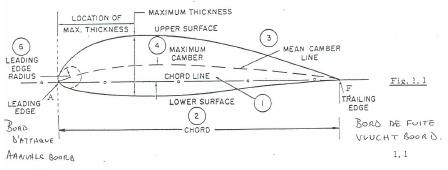
\includegraphics[scale=1]{ch2/1}
		\captionof{figure}{}
		\end{center}
		
		The connection between the trailing edge and the leading edge is called the \textbf{chord}. Then we have a \textbf{camber line} which is the line following the shape of the airfoil and characterizing the geometry. The leading and trailing edges are respectively the starting and ending point of the camber line. The thickness is always normal to the camber line. Let's note that the camber line and the thickness distribution are function of the position $f(x)$. \\
		
		Eastman Jacobs created around 1930 a family of wing profiles, known as the NACA profiles. He characterised them by 4 digit numbers: 
		
		\begin{itemize}
			\item[•] The first is the \textbf{maximum camber in percentage of the chord} 
			\item[•] The second is the \textbf{position of the maximum camber in 1/10 percentage of the chord}
			\item[•] The last two digits gives the \textbf{position of the maximum thickness in percentage of the chord}\\
		\end{itemize}				
		
		These were characterizing the 2D representation, but a wing is 3D. We have also the \textbf{wing surface S}, \textbf{the span of the wing b} and we can define a mean chord when this last is not constant as: 
		\begin{equation}
		<c> = \frac{S}{b}.
		\end{equation}				
		 For civil aircraft, b/c is between 6-10 and for glider b/c = 12, this is called the \textbf{aspect ratio} (slenderness ratio). 
		 
		 \newpage
		 
	\section{The flow around 2D airfoils}
		
		\begin{wrapfigure}[9]{l}{7.5cm}
		\vspace{-5mm}
		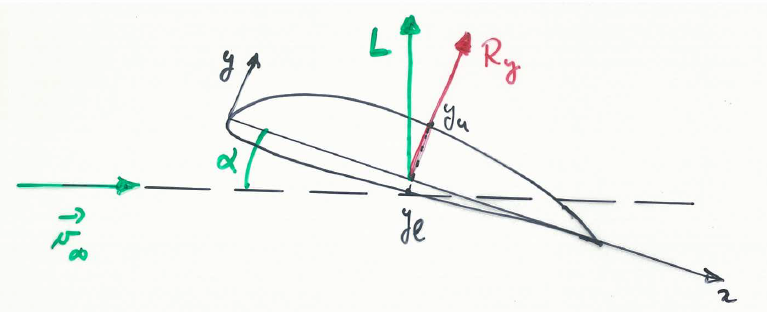
\includegraphics[scale=0.35]{ch2/3}
		\captionof{figure}{}
		\label{fig:2.2}
		\end{wrapfigure}
		Let's remind the expression of the force applied on the wing:
		
		\begin{equation}
		\vec{R} = -\oint p \, d\vec{S} + \oint \bar{\bar{\tau}} \, d\vec{S} 
		\end{equation}
		
		with an external normal to the airfoil. The angle of attack is represented on \autoref{fig:2.2}.

		The pressure term is responsible for lift and the friction term is responsible for drag. Friction forces work tangential to the airfoil and the pressure forces are perpendicular, if there is \textbf{no separation} in the flow. The drag created by the stress is called the \textbf{skin} or \textbf{friction} drag. 
		Note that in a subsonic inviscid incompressible flow, we have the paradox of d’Alembert because we have no drag. This shows that the pressure only contributes to lift. \\

		What happens when we have \textbf{separation} is that we have a region above the airfoil where $p-p_\infty \approx 0$ and so we have a very big pressure below $p\gg p_\infty$ that slows down the wing. This implies that the applied force is higher than the case without separation and due to the attack angle, the drag force too. This phenomenon is called \textbf{pressure drag} (form drag), and here the pressure contributes to drag.
		
		\begin{center}
		ADD FIGURE 4
		\end{center}
		
		\begin{wrapfigure}[15]{r}{6cm}
		\vspace{-5mm}
		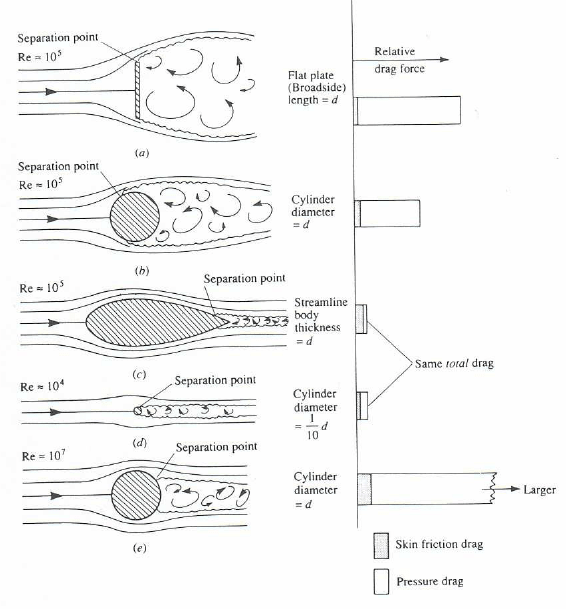
\includegraphics[scale=0.4]{ch2/2}
		\captionof{figure}{}
		\end{wrapfigure}
		The figure shows how the geometry of the body influence the drag force which can be sometimes principally caused by pressure. If we have a flat plate or a cylinder we have a huge separation, so principally a form drag $D_f$. We will have less pressure drop with the wing profile as it perfectly follows the flow direction, to end up smoothly, in this case the friction drag $D_f$ is more important. This shows the importance of profiles. \\
		
		If we look to the weight of a plane, it is surprising to see the importance of lift force. This is possible thanks to the high \textbf{atmospheric pressure}. Indeed, the wing load is defined as: 
		
		\begin{equation}
		\mbox{wing load} = \frac{\mbox{weight plane}}{\mbox{surface aera wings}}
		\end{equation}
				
		and this is commonly approximately equal to 5000 Pa = 500 $kg/m^2$. This can be easely reached by a small perturbation of the atmospheric pressure ($10^5$Pa $\rightarrow$ $5\% = 5000$ Pa). \\
		
		\subsection{Distribution of the pressure coefficient}
			Let's see the effect of the angle of attack. For small angles, we can neglect the force derivation implied and consider it to be perpendicular to the chord. This allows to neglect the drag component (refer to \autoref{fig:2.2}). If we assume that $v$ is in the x direction, the lift force approximation is:
			
			\begin{equation}
			R_y = - \oint p \, d\vec{S}.\vec{1}_y = - \oint p \, dS_y.
			\end{equation}						
			 
			The lift force is fully created by pressure and we can call the lower part of the wing the \textbf{pressure side} and the upper part the \textbf{suction side}. 
			
			\begin{wrapfigure}[11]{l}{8cm}
			\vspace{-5mm}
			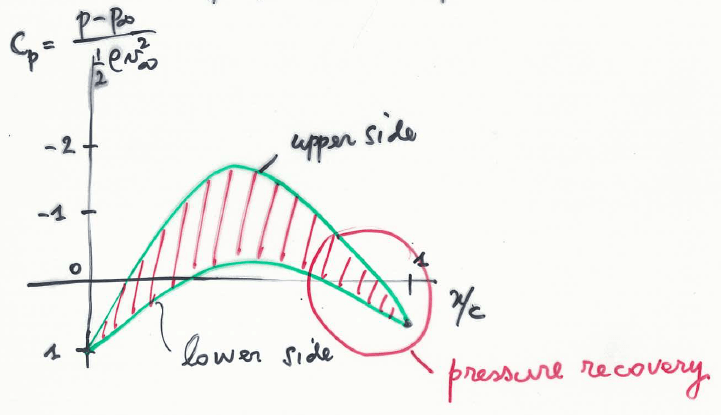
\includegraphics[scale=0.4]{ch2/4}
			\captionof{figure}{}
			\label{fig:2.4}
			\end{wrapfigure}
			The suction effect is always bigger than the pressure one. We introduce the pressure coefficient $C_p = \frac{p-p_\infty}{\frac{1}{2}\rho v_\infty ^2}$ which direction points always down! The pressure side is the green curve below and the suction side is the green curve on the upper side of \autoref{fig:2.4}. \\

			If we look to the leading edge, we have a tendency to go to $C_p = 1$. Indeed, if we write Bernouilli along a streamline and take into account the stagnation point where $v=0$, we have:
			
			\begin{equation}
			p_\infty + \rho \frac{v_\infty ^2}{2} = cst = p_{LE} + 0 \qquad \Rightarrow C_p = \frac{p_{LE}-p_\infty}{\frac{1}{2}\rho v_\infty ^2} = 1.
			\end{equation}						
			
			The pressure recovery means that we will have again $p = p_\infty$ at that point. At the leading edge this is the case because it is commonly a stagnation point. \\ 

For the trailing edge we have two cases. If it is \textbf{blunt} trailing edge, we have the $C_p = 1$ case (leading edge always blunt). If we have a \textbf{sharp} trailing edge, we will have $v_\infty$ at the previous stagnation point and so the Bernouilli equation rewrites:

			\begin{equation}
			p_\infty + \cancel{\rho \frac{v_\infty ^2}{2}} = cst = p_{TE} + \cancel{\rho \frac{v_\infty ^2}{2}} \qquad \Rightarrow C_p = \frac{p_{TE}-p_\infty}{\frac{1}{2}\rho v_\infty ^2} = 0.
			\end{equation}
			
			\begin{wrapfigure}[7]{r}{8cm}
			\vspace{-5mm}
			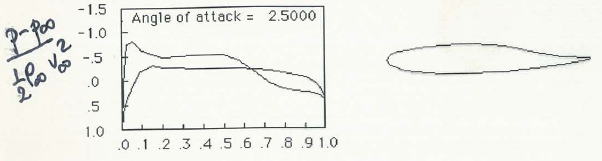
\includegraphics[scale=0.5]{ch2/5}
			\captionof{figure}{}
			\end{wrapfigure}
			We have a very big expansion on the LE (separation), so this induces a suction peak as the pressure falls above and increases below. Then we go back to the normal pressure. Let’s remind that decreasing pressure is favourable because the flow stays attached but if we have pressure increase, it's unfavourable, because we risk separation.
The angle of attack is important because the flow has more difficulties to turn on the LE  when angle goes up so the separation and the sucking peak are more important.\\

			This case is particular because the rear is reversed, so the pressure side becomes sucking and inversely. The reduced camber and reduced thickness makes the wing more vulnerable to angle change.
			
			\begin{wrapfigure}[2]{l}{7.5cm}
			\vspace{-5mm}
			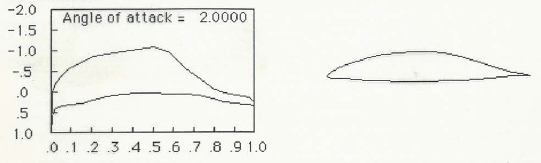
\includegraphics[scale=0.5]{ch2/6}
			\captionof{figure}{}
			\end{wrapfigure}
			Natural laminar section. The smoother LE reduces the peak and the sharp TE induces $C_p = 0$.\\\\
			
			\begin{wrapfigure}[2]{r}{7.5cm}
			\vspace{-5mm}
			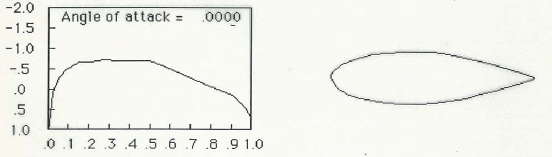
\includegraphics[scale=0.5]{ch2/8}
			\captionof{figure}{}
			\end{wrapfigure}
			This is a symetrical shape and thus only one line is shown. The thickness makes it more resistible to angle change. \\\\\\
			
			\begin{wrapfigure}[2]{l}{7.5cm}
			\vspace{-5mm}
			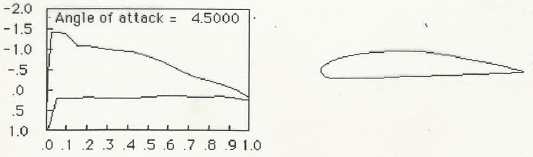
\includegraphics[scale=0.5]{ch2/9}
			\captionof{figure}{}
			\end{wrapfigure}
			Even if the wing is thin, the camber makes it more suited to high attack angle. \\\\\\
		
		\section{Center of pressure, moment and aerodynamic center}
			\subsection{Center of pressure and moment}
				\subsubsection{Calculation of lift force}
					\begin{wrapfigure}[12]{r}{3.5cm}
					\vspace{-5mm}
					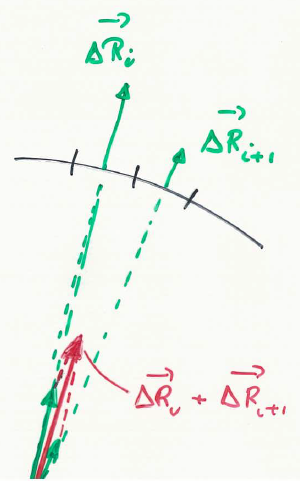
\includegraphics[scale=0.4]{ch2/10}
					\captionof{figure}{}
					\end{wrapfigure}
					We can calculate the lift by $L = \rho v_\infty \Gamma$, but we need the $\Gamma$ which is not calculable. So we will use the trick that consist in forgetting the drag term in the $\vec{R}$. Then we integrate the pressure around the surface:
					
					\begin{equation}
					\vec{R} = -\oint p \, d\vec{S} = - \sum \underbrace{p_i \vec{\Delta S_i}}_{\Delta R_i}
					\end{equation}
					
				\subsubsection{Center of pressure}
					It's the x value on the chord where the carrier of the force $\vec{R}$ intersects the chord. It's function of the angle of attack. Indeed, if alpha increases, the suction peak will be higher, this induces that the center of pressure move forward (participation of the forward pressure more important).\\
					
					Note that the center of pressure is not a fixed point. Indeed, it varies with the angle of attack: if $\alpha \nearrow$, the pressure peak on the LE is more important making the $x_p$ move upstream, and the contrary for $\alpha \searrow$. This notion will be completed by the \textbf{zero lift angle} $\alpha _{0}$.
					
				\subsubsection{Equivalent forces}
					\begin{wrapfigure}[7]{l}{3cm}
					\vspace{-5mm}
					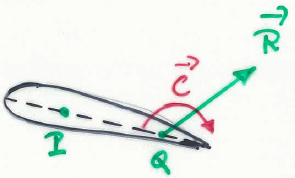
\includegraphics[scale=0.4]{ch2/11}
					\captionof{figure}{}
					\end{wrapfigure}
					The force at the pressure center P is equivalent to another force in point Q, but by adding the moment to compensate the one added by moving the force. This moment is:
					
					\begin{equation}
					\vec{C_Q} = -\vec{PQ}\times \vec{R}.
					\end{equation}
					
				\subsubsection{Aerodynamic center}
					Suppose that there is a point Q where this couple $C_Q$ is independent of the angle of attack (because the pressure center changes with alpha). This point is called the aerodynamic center. We have to show that this exists. For this way:
					\begin{enumerate}
						\item We will begin by calculating the center of pressure by integrating the pressure field. We can calculate the magnitude, but not the acting point. 
						
						\item We compute the momentum of the pressure forces around the leading edge (\autoref{fig:2.11}):
						
						\begin{equation}
						\vec{M}_{LE} = \oint \vec{OQ} \times d\vec{F} = \underbrace{M_{LE}}_{<0} \vec{1}_z 
						\end{equation}
						where $\vec{1}_z$ goes in the paper. 						
						
						\item On the other hand, we know that $\vec{R}$ has a certain direction with a normal component, so we can make the moment (\autoref{fig:2.12}): 
						
						\begin{equation}
						M_{LE} = -x_p.N
						\end{equation}
					\end{enumerate}
					
					By using point 2 and 3 we can find $x_{p}$.
					
					\begin{center}
					\begin{minipage}{0.4\textwidth}
					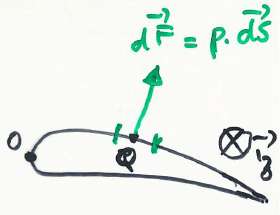
\includegraphics[scale=0.65]{ch2/12}
					\captionof{figure}{}
					\label{fig:2.11}
					\end{minipage}
					\begin{minipage}{0.4\textwidth}
					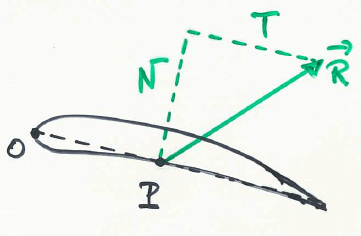
\includegraphics[scale=0.6]{ch2/13}
					\captionof{figure}{}
					\label{fig:2.12}
					\end{minipage}
					\end{center}
					
		\subsection{Aerodynamic center}
			Let's now be interested in how the the moment on a point Q on the wing varies with $\alpha$. It is shown experimentally that:
			
			\begin{equation}
			c_m(Q) = c_{m_0} + k c_l
			\label{eq:2.11}
			\end{equation}
			
			where $c_m, c_l$ are respectively the non-dimensional moment and lift, and $c_{m_0}$ the non-dimensional moment at zero lift. $k$ is a constant that is related to the reference point chosen. If $Q$ is taken on the LE for example, increasing $\alpha$ will produce an increase of the lift and make the center of pressure move upstream. The L increase will compensate the moving $x_p$ such that the moment becomes even more noose-down (more negative following $\vec{1}_z$) $\Rightarrow k<0$ for a decrease in \eqref{eq:2.11}. The same reasoning applied on the trailing edge gives $k>0$. \\
			
			This shows that it exists a point where $k = 0$, called the \textbf{aerodynamic center}. According to \eqref{eq:2.11}, this point will have a constant moment whatever $\alpha$. Indeed, we will show that $c_l = m(\alpha - \alpha _0)$ and so:
			
			\begin{equation}
			c_m(Q) = c_{m_0} + k m(\alpha - \alpha _0) \qquad \Rightarrow c_m(Q) = c_{m_0}.
			\end{equation}			 
			
			We can benefit from this equation to show that $c_{m_0}$ is well the moment for $\alpha = \alpha _0$, the zero lift angle (negative, descending arrow). We will also later show that when we decrease the angle of attack beginning from a positive one to the zero lift angle, the $x_p$ will go downstream till infinity away the trailing edge, with an infinitely small lift,. This means that we will always have a finite noose-down moment. \\
			
			Taking the opposite case of beginning from negative value of $\alpha$, we will have the same value since the lift force is negative and the $x_p$ in infinity further away from the leading edge. The \textbf{moment at zero lift} is thus \textbf{negative}. The explanations lead to the figures below.
			
			\begin{center}
			\begin{minipage}{0.33\textwidth}
			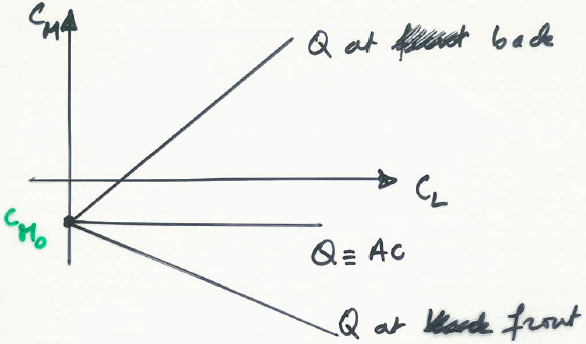
\includegraphics[scale=0.33]{ch2/14}
			\captionof{figure}{}
			\end{minipage}
			\begin{minipage}{0.32\textwidth}
			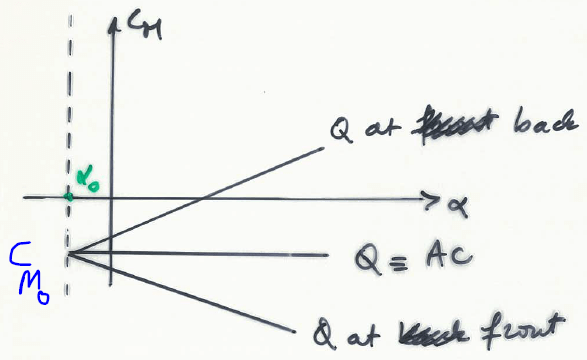
\includegraphics[scale=0.32]{ch2/15}
			\captionof{figure}{}
			\end{minipage}
			\begin{minipage}{0.32\textwidth}
			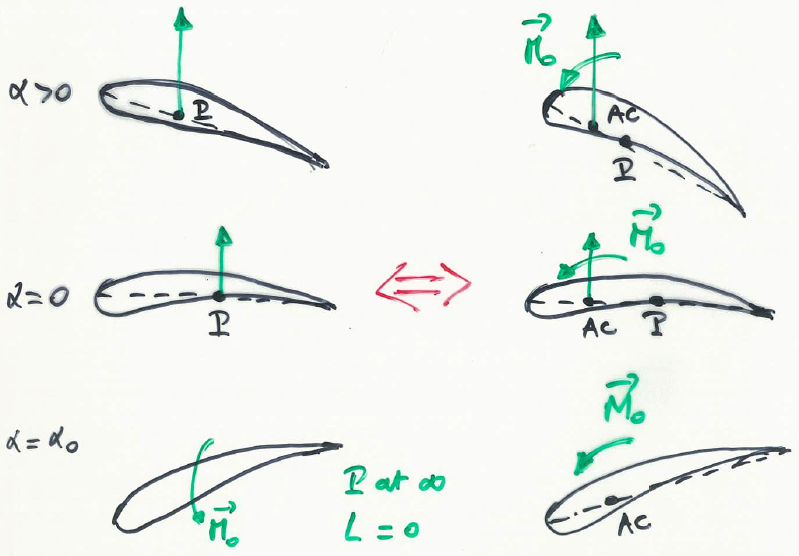
\includegraphics[scale=0.21]{ch2/16}
			\captionof{figure}{}
			\end{minipage}
			\end{center}
		
			\begin{wrapfigure}[8]{l}{4.5cm}
			\vspace{-5mm}
			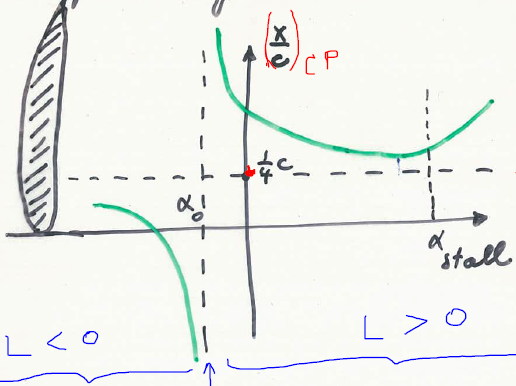
\includegraphics[scale=0.3]{ch2/17}
			\captionof{figure}{}
			\end{wrapfigure}
			Let's finally establish the evolution of the pressure center in function of $\alpha$. For this purpose, we need 4 equations:
			
			\begin{equation}
			\begin{array}{cccc}
			1) & c_m = c_{m_0} + kc_l & 2)& M_{ac} = (x_{ac}-x_{cp})N \\
			3) & m_{ac} = M_{AC} = M_0 <0 & 4) & N = n(\alpha-\alpha _0)
			\end{array}
			\end{equation}
		
		 	The AC being always upstream the CP the difference in 2) is $<0$. In 4), $n>0$. By using equation 3,4 and 2, we can compute:
		 	
		 	\begin{equation}
		 	M_0 = -(x_{cp}-x_{ac}).n(\alpha - \alpha _0) \quad \Leftrightarrow \quad -\frac{M_0}{n} = (x_{cp}-x_{ac}).(\alpha - \alpha _0)
		 	\end{equation}
		 	
		 	This is the equation of an \textbf{hyperbola}. To see it, we only have to compute the limits of:
		 	
		 	\begin{equation}
		 	\begin{array}{c}
		 	x_{cp} = x_{ac} - \frac{M_0}{n}\frac{1}{\alpha - \alpha _0}\\
		 	\lim _{\alpha \rightarrow \pm\infty} x_{cp} = x_{ac} \qquad \lim _{\alpha \rightarrow \alpha _0 >0} x_{cp} = +\infty \qquad \lim _{\alpha \rightarrow \alpha _0 <0} x_{cp} = -\infty
		 	\end{array}
		 	\end{equation}
		 	
		 	The graph is shown on figure. Let's finally say that commonly, $x_{ac} = cst \approx \frac{1}{4}C$.\\
		 	
		 	 A particular case is the one of \textbf{symmetrical profile}. Indeed, in that case, the $\alpha _0$ case correspond to $M_{ac} = 0$ and $L=0$. The pressure center corresponds with the aerodynamic center and is \textbf{fixed}.  
		 	 
	\section{2D characteristics}
		\subsection{Lift, drag and moment curves}
			Let’s look to the non-dimensional parameters that will influence the lift;, the drag and the momentum. We have to define some reference quantities: 

			\begin{equation}
			\begin{array}{cccc}
			L_{ref} = C & v_{ref} = v_\infty & t_{ref} = L_{ref}/v_{ref} & \rho _{ref} = \rho _\infty \\
			t’= t/t_{ref} & p_{ref} = \rho _{ref} \frac{v_{ref} ^2}{2} & \mbox{Mach} = V_{ref} / a_{ref} & a_{ref} = \gamma \pi T_{ref} \\
			\gamma = c_p / c_v && Re_{ref} = \frac{\rho _{ref} v_{ref} L_{ref}}{\mu _{ref}} &
			\end{array}
			\end{equation}					
			
			where $a$ is the speed of sound. By replacing all these in the mass, momentum and energy equations, we obtain the non-dimensional ones (see Fluid Mechanics II):
			
			\begin{equation}
			\begin{aligned}
			&\bullet\frac{\D \rho '}{\D t'} + \nabla \left(\rho ' \vec{v}'\right) = 0\\
			&\bullet\rho ' \frac{d\vec{v}'}{dt'} = - \frac{1}{\gamma M^2_{ref}}\nabla p' + \frac{1}{\mbox{Re}_{ref}}\nabla \bar{\bar{\tau}'}\\
			&\bullet\frac{d}{dt'}(\rho ' e')+ \frac{\gamma (\gamma -1)}{2} M^2_{ref}\frac{d}{dt'}(\rho ' \vec{v'}^2 ) \\
			&= \frac{\gamma}{Pr_{ref}Re_{ref}} \nabla (k'\nabla T') - (\gamma -1)\nabla (p'\vec{v}')+ \gamma (\gamma -1) \frac{M_{ref}^2}{Re_{ref}} \nabla (\bar{\bar{\tau}}'\vec{v}')			\end{aligned}
			\end{equation}
		
			We can see that a solution can only be function of 4 parameters: $M, Re, Pr = \frac{c_p \mu}{k}, \gamma$, but we know that the geometry and the angle of attack $\alpha$ have a role by means of the boundary conditions. Then, we assume that the fluid is air ($\gamma =1.4$) and that we can neglect heat effects (no influence of Pr, incompressible and so low speed flows). The non-dimensional lift, drag and moment are thus function of M, Re, geometry and $\alpha$. We can define \textbf{lift}, \textbf{drag} and \textbf{moment coefficient} as (we forget about compressibility $\rightarrow$ M, and Re effects are low for $C_L and C_M$): 
			
			\begin{equation}
			\begin{aligned}
			&C_L(\cancel{M}, \cancel{Re}, geometry, \alpha) = \frac{L}{\frac{1}{2}\rho _{ref} v^2_{ref} S} \\
			&C_D(\cancel{M},Re, geometry, \alpha) = \frac{D}{\frac{1}{2}\rho _{ref} v^2_{ref} S}		\\
			&C_M(\cancel{M}, \cancel{Re}, geometry, \alpha) = \frac{M}{\frac{1}{2}\rho _{ref} v^2_{ref} Sc}
			\end{aligned}	
			\label{eq:2.18}		
			\end{equation}
			
			where L, D, M are the \textbf{dimensional} forces, c the mean chord (S/b) and S a reference surface (3D wing $\rightarrow$ total wing surface, 2D wing $\rightarrow$ S = c). We can experimentally show that the lift increases mainly linearly with $\alpha$ and the drag force is caused by friction effects and pressure differences involving with $\alpha$. This gives the following equations (lower case for 2D):
			
			\begin{equation}
			c_l = m(\alpha - \alpha _{L_0}) \qquad c_d = c_{d_0} + kc^2_l
			\end{equation}
			
			where $m\approx 2\pi$ theoretically and 5.7 practically, k is a constant of order of magnitude 0.01. 
			
		\subsection{Stall and critical angle of attack}
			\begin{wrapfigure}[11]{l}{6cm}
			\vspace{-5mm}
			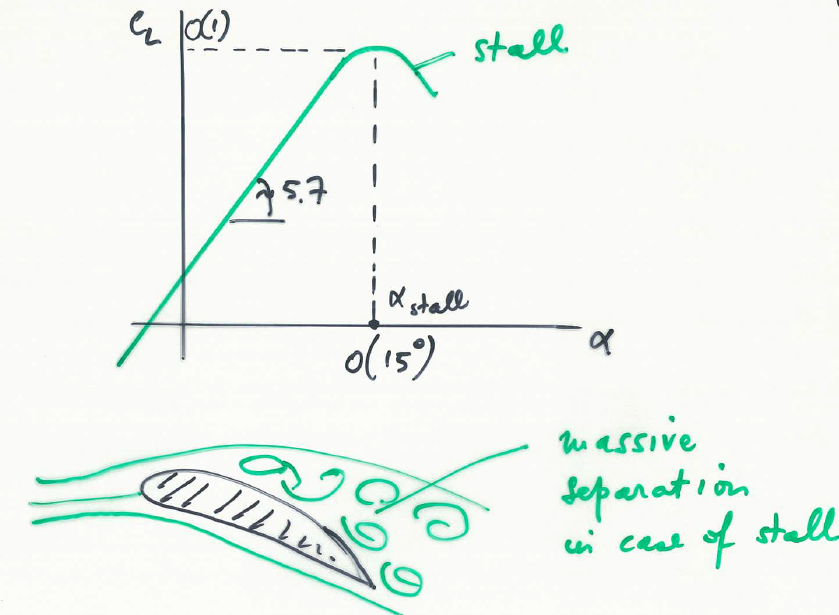
\includegraphics[scale=0.26]{ch2/18}
			\captionof{figure}{}
			\end{wrapfigure}
			At a certain angle of attack ($\approx 15\degres$), the lift suddenly drops. This is due to massive separation on the suction side (reverse pressure gradient too high) and happens at the \textbf{critical angle of attack}. This phenomenon is called \textbf{stall}. In the separated part, the pressure will no longer decrease and will form a pressure plateau. \\
			
			We have to make the difference between leading-edge stall and trailing-edge stall. For \textbf{leading-edge stall}, the massive separation occurs suddenly near the LE resulting \newpage
			
			\begin{wrapfigure}[13]{r}{5.7cm}
			\vspace{-5mm}
			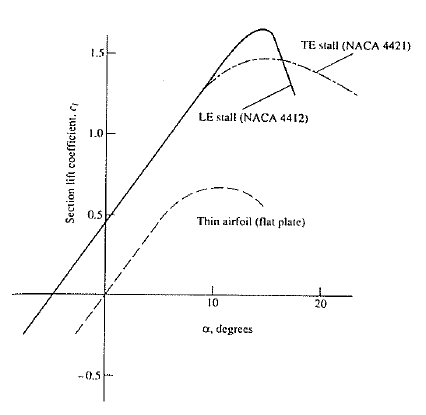
\includegraphics[scale=0.5]{ch2/19}
			\captionof{figure}{}
			\end{wrapfigure}
			in a strong and sudden drop of lift, when at maximum lift. This especially occurs to thin airfoils with cross-sections between 10 and 16\% of the chord. For the \textbf{trailing-edge stall}, the point of separation gradually goes upstream with increasing angle of attack resulting in a more gradual drop of lift (more thick airfoils). The comparison is done on the right figure. We can also see a third type of stall called \textbf{thin airfoil stall} with the example of a flat plat.  \\
			
			In conclusion, the LE must be sufficiently rounded to have a good maximum lift. In fact the profile may nor be too 
			
			\begin{wrapfigure}[8]{l}{7cm}
			\vspace{-5mm}
			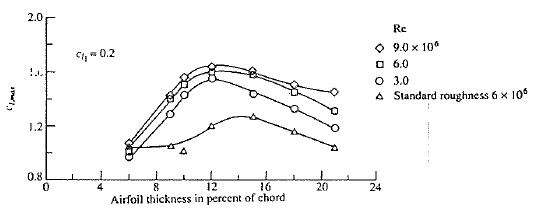
\includegraphics[scale=0.5]{ch2/20}
			\captionof{figure}{}
			\end{wrapfigure}
			thick  nor too thin. The figure on the left shows the influence of the thickness on the lift. We notice that the optimum thickness is situated around 12\% of the chord.The maximum lift increases with RE, indeed higher the Re, higher is the ratio of speed versus viscosity. So we can better oppose to separation. Unlike the Re number, the roughness has great effects on the maximum lift. Finally, let's notice that the camber have also an effect on maximum lift, the best is a camber of 8 up to 10\%. 
			
		\subsection{Maximum lift, stalling speed, polar curve and glide ratio}
			From $C_L$ in \eqref{eq:2.18}, we can deduce the lift:
			
			\begin{equation}
			L = C_L \frac{1}{2} \rho _{ref} v^2_{ref} S.
			\label{eq:2.21}
			\end{equation}
			
			The lift force must always at least be equal to the weight of the plane. This implies that for low speed (take-off and landing), the $C_L$ must be large. This is accomplished with large $\alpha$ and slats or flaps. The minimum speed where the lift can still balance the weight ($C_L$ maximum) is called \textbf{stall speed} and from \eqref{eq:2.21} we find:
			
			\begin{equation}
			v_{stall} = \sqrt{\frac{W}{C_{L_{max}} \frac{1}{2} \rho_{ref} S}}
			\end{equation}
			
			\begin{wrapfigure}[10]{r}{4cm}
			\vspace{-5mm}
			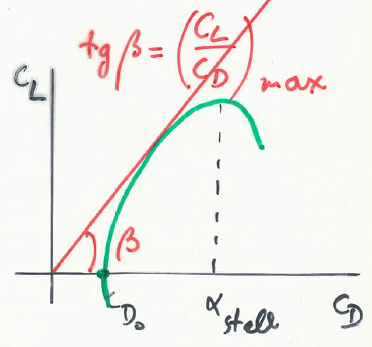
\includegraphics[scale=0.4]{ch2/21}
			\captionof{figure}{}
			\end{wrapfigure}
			The curve that represents $C_L$ in function of $C_D$ is the \textbf{polar curve} of the wing. The ratio $\frac{C_L}{C_D}$ is the \textbf{glide ratio} or \textbf{finesse} and is like an efficiency parameter. The best parameter is obtained using the graph by calculating $\beta$ such that: 
			
			\begin{equation}
			\tan \beta = \left(\frac{C_L}{C_D}\right)_{max}
			\end{equation}						
			 
			This point is important for the quality of the wing because if we plot the thrust, the lift, the drag and the weight of a plane describing a horizontal flight (\autoref{fig:2.21}), the thrust is given by:
			
			\begin{equation}
			T = \frac{L}{\tan \beta} = \frac{W}{\tan \beta}
			\end{equation}
			
			where we see that when $\tan \beta$ (so the glide ratio) increases, T decreases. Another interpretation can be given when we have no thrust (\autoref{fig:2.22}). In this case the gliding ratio has to be adapted to travel the larger distance knowing that:
			
			\begin{equation}
			\frac{C_L}{C_D} = \frac{\mbox{distance travelled}}{\mbox{height loss}}
			\end{equation}
			
			\begin{center}
			\begin{minipage}{0.3\textwidth}
			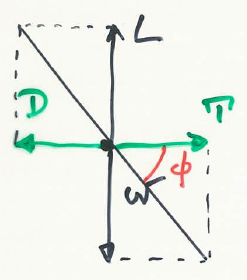
\includegraphics[scale=0.6]{ch2/22}
			\captionof{figure}{}			
			\label{fig:2.21}
			\end{minipage}
			\begin{minipage}{0.5\textwidth}
			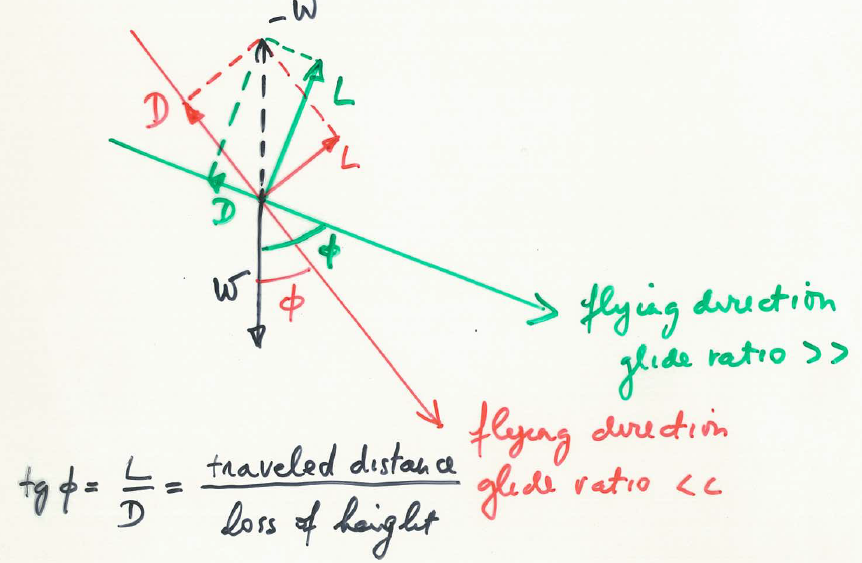
\includegraphics[scale=0.3]{ch2/23}
			\captionof{figure}{}			
			\label{fig:2.22}
			\end{minipage}
			\end{center}
			
\section{Methods to calculate flows around 2D airfoils}
	\subsection{Conformal mapping}
		We will begin here with steady, inviscid irrotational flows. This gives for the mass conservation equation:
		
		\begin{equation}
		\frac{\D \rho}{\D t} + \nabla (\rho \vec{v}) = 0 \qquad \Rightarrow \nabla \vec{v} = 0 = \D _x u + \D _y v
		\end{equation}
		
		In the other hand, we have the assumption of irrotational flow:
		
		\begin{equation}
		\vec{w} = 0 \qquad \Rightarrow \D _x v - \D _y u = 0.
		\end{equation}
		
		Then we define the \textbf{complex potential functoin w}:
		
		\begin{equation}
		w = \phi + I\psi
		\end{equation}		 
		
		where $\phi$ is the \textbf{potential function} (satisfies $w=0$ by construction) such that:
		
		\begin{equation}
		\left\{
		\begin{aligned}
		&u = \D _x \phi \\
		&v = \D _y \phi
		\end{aligned}
		\right.
		\qquad
		\nabla \phi = \vec{v} = \D _x\phi \vec{1} _x + \D _y \phi \vec{1}_y
		\end{equation}
		
		We must satisfy the mass conservation equation:
		\begin{equation}
		\nabla (\nabla \phi) = 0 \qquad \Rightarrow \Delta \phi = 0 
 		\end{equation}
 		
 		coupled with boundary conditions, we can find a solution $\phi (x,y)$. The \textbf{stream function} satisfies the mass conservation by construction:
 		
 		\begin{equation}
 		\left\{ 
 		\begin{aligned}
 		&u = \D _y \psi\\
 		&v = - \D _x \psi
 		\end{aligned}
 		\right.
 		\qquad \Rightarrow \D _x u + \D _y v = 0 \Leftrightarrow \D _x (\D _y \psi) + \D _y (- \D _x \psi) = 0
 		\end{equation}
 		
 		\begin{wrapfigure}[10]{l}{5cm}
		\vspace{-5mm}
		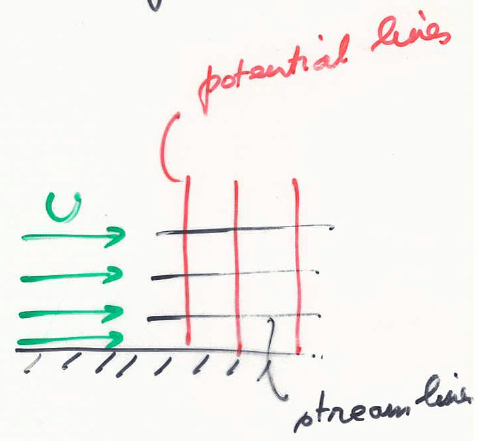
\includegraphics[scale=0.4]{ch2/24}
		\captionof{figure}{}
		\end{wrapfigure}
		We still have to verify the $w=0$ condition:
 		\begin{equation}
 		\D _x v - \D _y u = 0 \qquad \Rightarrow \frac{\D ^2 \psi}{\D x^2} + \frac{\D ^2 \psi}{\D y^2} = 0 \qquad \Delta \psi = 0
 		\end{equation}
 		A streamline and a potential line are perpendicular to each other:
 		\begin{equation}
 		\nabla \psi . \nabla phi = \D _x \psi \D _x \phi + \D_ y \psi \D _y \phi = -vu + uv = 0. 
 		\end{equation}